\section{Background and Motivation}\label{sec:background}

\subsection{RGNN Formulation and Operators}
\label{sec:rgnn_formulation}



RGNNs extend GNNs to model different node and edge types for relational graph data.
For example, extended from GCN, a relational graph convolutional network~(RGCN) layer is defined as 
\begin{equation} \label{eq:rgcn}
     \overrightarrow{{h}_v^{(l+1)}} = \sigma\left(\overrightarrow{{h}_v^{(l)}}W_0^{(l)}+\sum_{r \in R}\sum_{u \in \mathcal{N}_v^r}\frac{1}{c_{v,r}}\overrightarrow{{h}_u^{(l)}}W_r^{(l)}\right)
\end{equation}
, where $\mathcal{N}_v^r$ denotes neighbors of node $v$ in relation $r \in R$, 
${h}_n^{(l)}$ is the $l$-th layer node representation of $n$. 
$W_r^{(l)}$ is the weight for relation $r$. $c_{v,r}$ is a problem-specific normalization factor.
Figure~\ref{fig:rgnn_layer} shows an example of how output features are produced in the message passing formulation equivalent to Formula~\ref{eq:rgcn}: 
The forward propagation of an RGNN layer could be divided into \textcircled{1} the edge message generation stage and \textcircled{2} the node aggregation stage.
For simplicity, we focus on the output feature $\overrightarrow{h_z^{(out)}}$ of node $z$: To obtain $\overrightarrow{h_z^{(out)}}$, \textcircled{1} a message $\overrightarrow{msg}$ is generated for each incoming edge, and \textcircled{2} the edge messages go through weighted aggregation and an activation function $\sigma$ to produce $\overrightarrow{h_z^{(out)}}$. 
Notably, to obtain the output feature of node $v$, the input feature of $v$ itself is applied to the $W_0^{(l)}$ and added to the transformed neighbor features. We call this a virtual self-loop because it could be seen as if each node now has a new edge to itself.



\begin{figure}[!b]
\centering
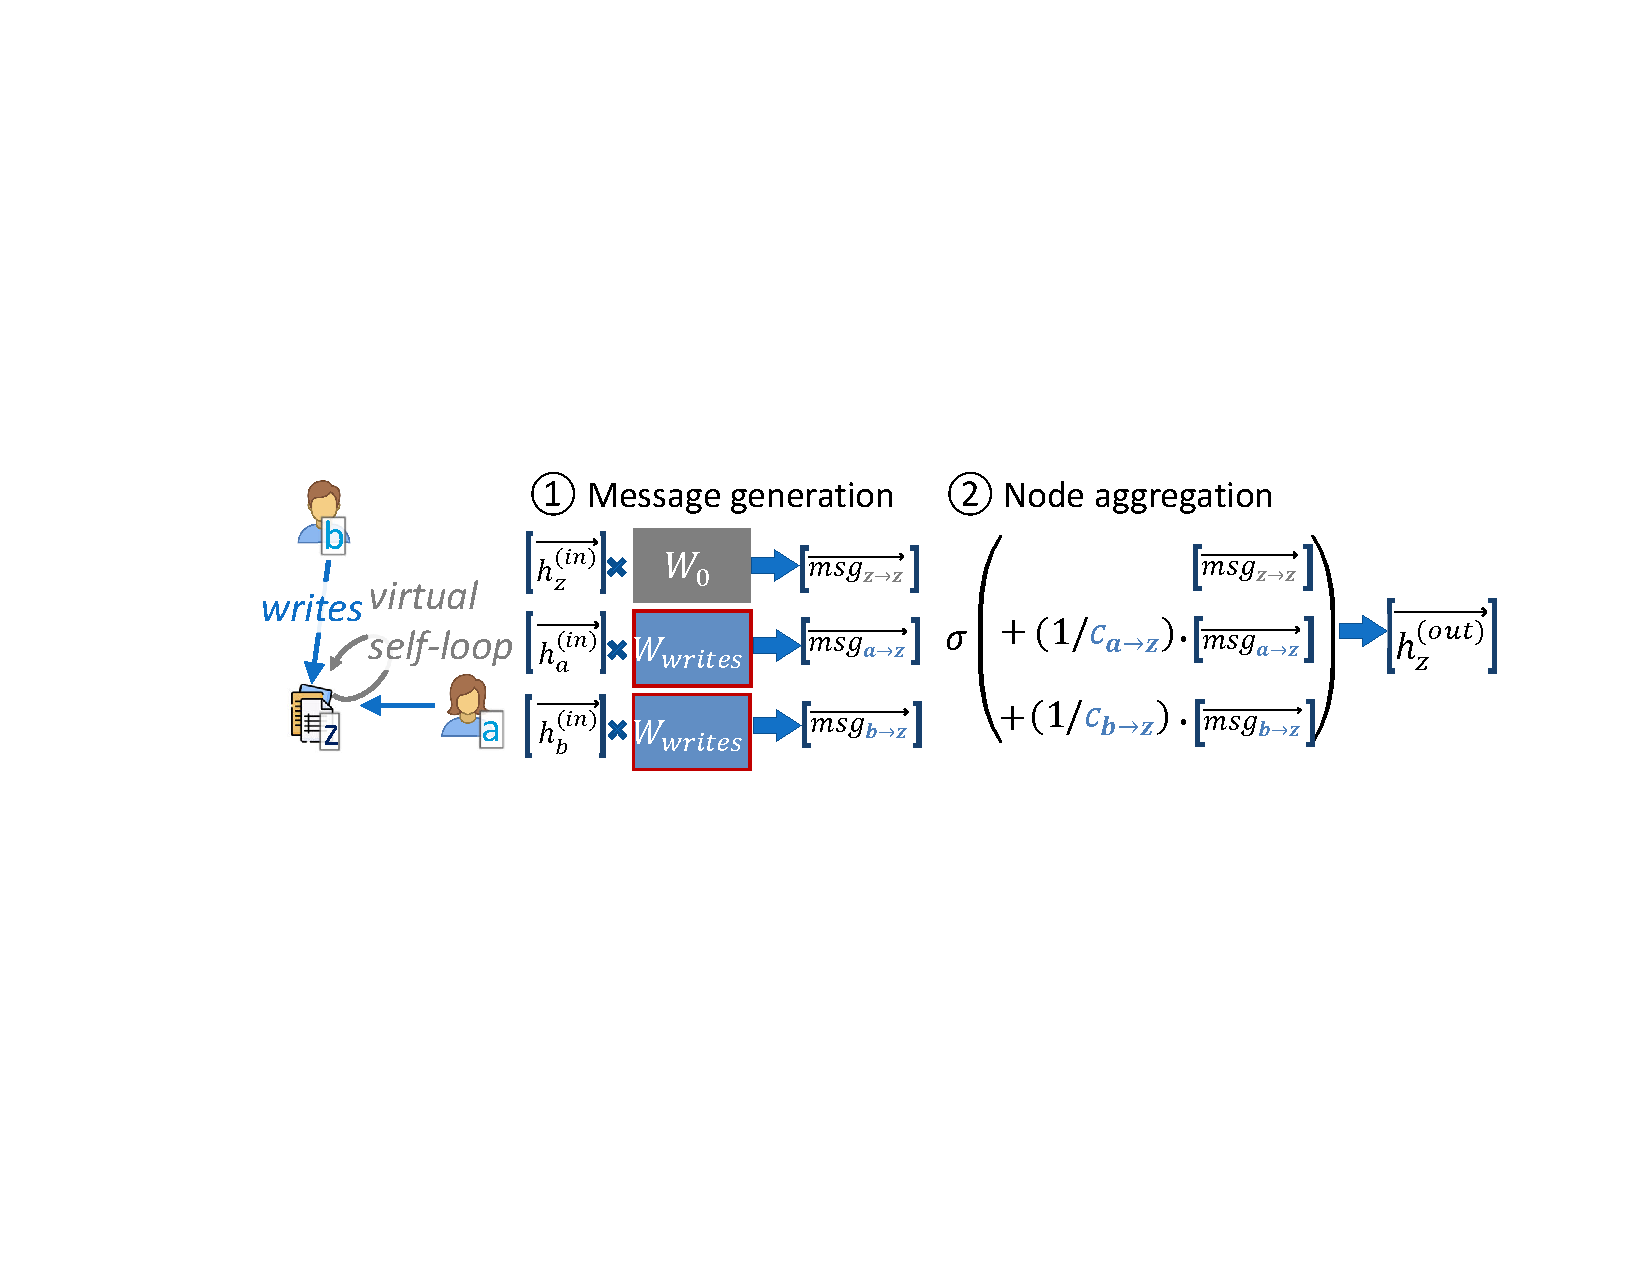
\includegraphics[width=\linewidth]{figures/Hector/RGCN_v3.pdf}
\caption{\label{fig:rgnn_layer} The forward propagation of an RGCN layer could be divided into \textcircled{1} message generation on edges and \textcircled{2} node aggregation. We focus on paper node $z$ in a large citation graph as an example. $z$ only has two incoming edges, from $a$ and $b$, respectively. $\overrightarrow{{h}^{(in)}}$ and $\overrightarrow{{h}^{(out)}}$ are node features. $W_{writes}$ is the weight for the type ``writes''. $W_{0}$ is the weight for virtual self-loops. $\sigma$ is the activation function. Notably, some runtime implementations may replicate data, e.g., $W_{writes}$. }
\end{figure}


\begin{figure}[!bt]
\centering
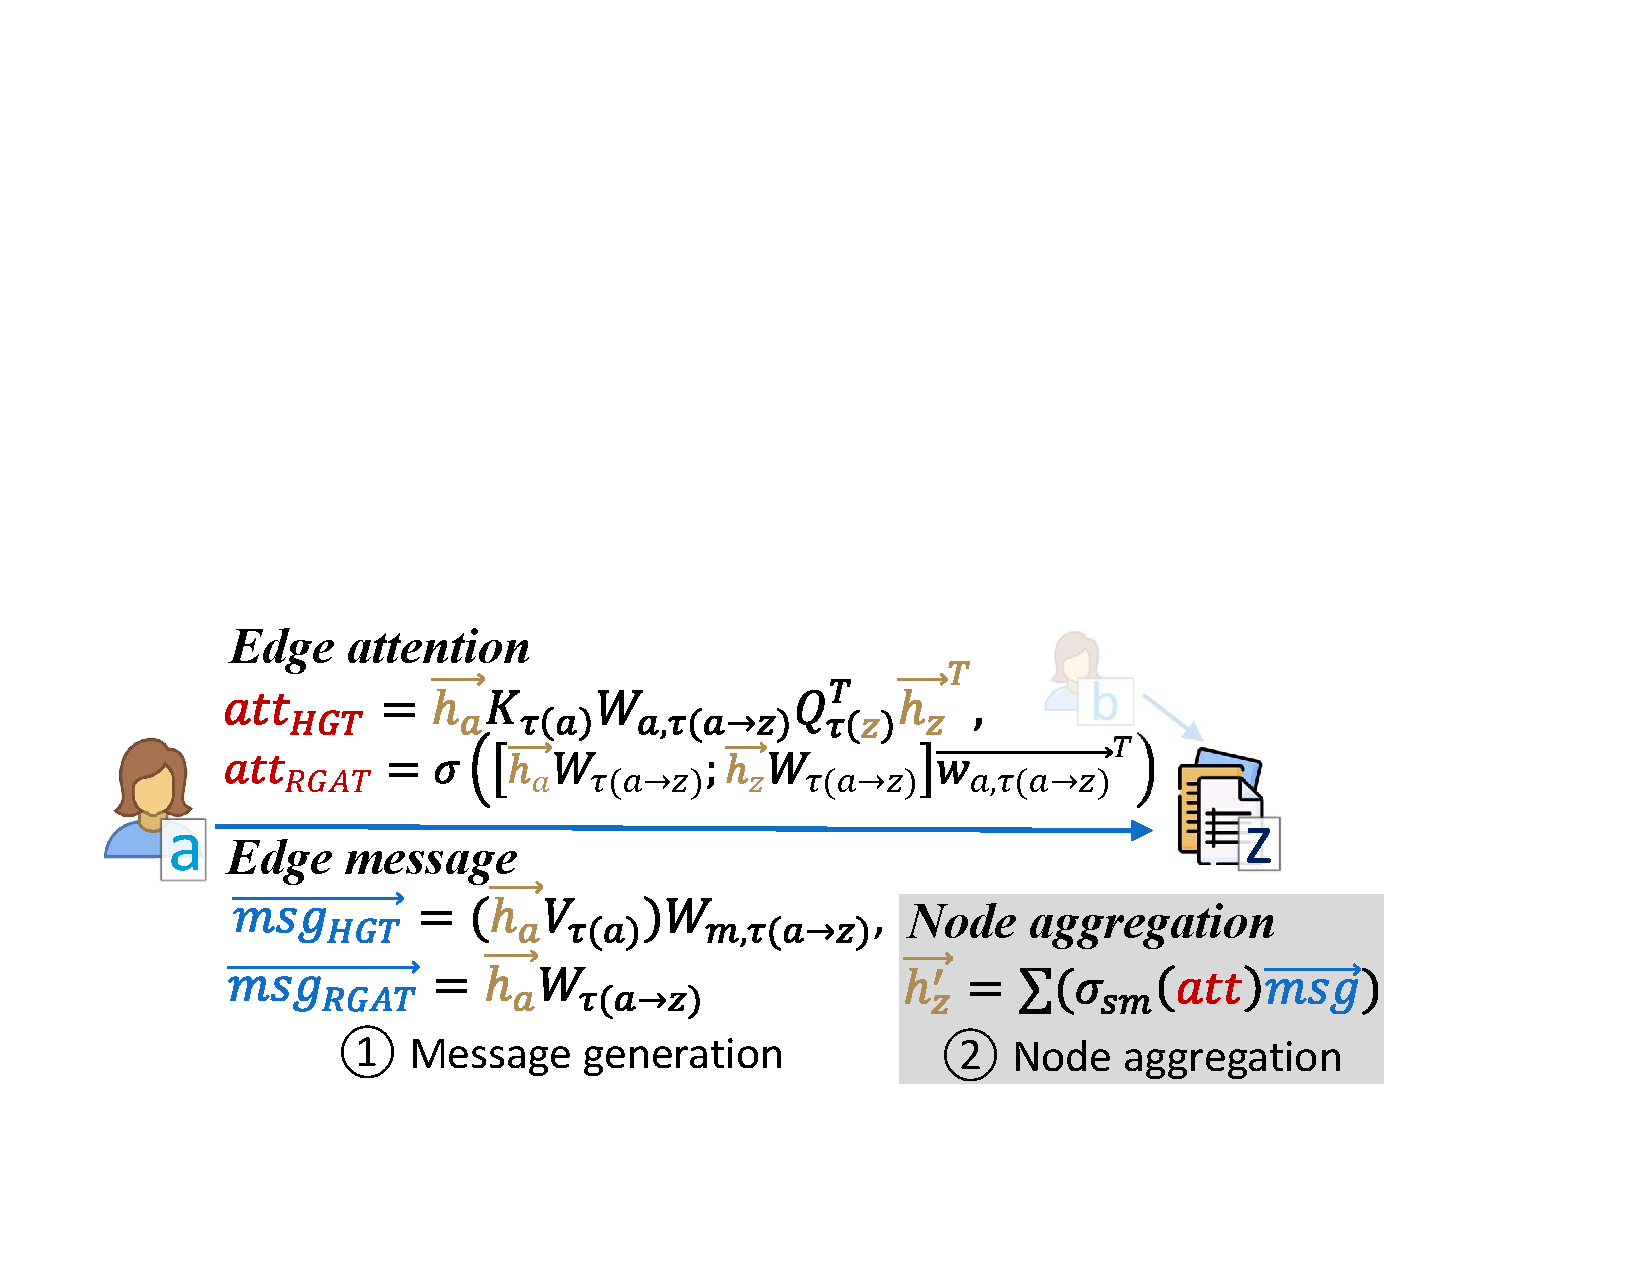
\includegraphics[width=0.8\linewidth]{figures/Hector/RGAT_HGT_v3.1.pdf}
\caption{\label{fig:rgat_layer} HGT and RGAT layer. $\overrightarrow{{h}_n}$ and $\overrightarrow{{h}_n^\prime}$ are node $n$'s features. Denote the type of edge from $a$ to $z$ as $\tau(a\rightarrow z)$. Weights $W_{a,\tau(a\rightarrow z)}$ differ by edge type $\tau(a\rightarrow z)$: For example, assuming there are two edge types, ``writes'' and ``cites'', $W_{a,\text{``writes''}}$ is a different weight from $W_{a,\text{``cites''}}$. They are defined and learned according to the edge type. $W_{m,\tau(a\rightarrow z)}$ and $\overrightarrow{{w}_{a,\tau(a\rightarrow z)}}$ are in similar situations. Weights $W_{\tau(n)}$ differ by the node type $\tau(n)$ of $n$. $\sigma$ is a leaky rectified linear unit~(ReLU) in the case of RGAT. $\sigma_{sm}$ stands for edge softmax. $[\vec{s};\vec{t}]$ concatenates $\vec{s}, \vec{t}$.}
\end{figure}

Relational graph attention network~(RGAT)~\cite{busbridge2019relational} and heterogeneous graph transformer~(HGT)~\cite{hgt} are shown in Figure~\ref{fig:rgat_layer}. Attention is introduced in these more complex models:
Attention is produced in the message generation stage together with edge messages.
Similar to the normalization factor, it is a scalar that emphasizes the message associated with the same edge during the subsequent node aggregation stage. However, attention is learned, as it is produced by operations among weights and features.

In addition to describing GNNs in two stages---message generation and node aggregation---a popular formulation uses the SpMM and SDDMM pair. The DGL~\cite{wang2019deep} paper has proven that GNN message passing can be expressed as generalized SpMM~(g-SpMM) and generalized SDDMM~(g-SDDMM) operations, with their backward propagation also following the same structure. SpMM computes the product of two matrices, $C=A\times B$, where the left matrix $A$ is sparse and in a sparse matrix format. The right matrix $B$ is dense. Notice that each row in $C$ is a weighted aggregation of specific rows in $B$ according to $A$:

\begin{equation*}
\overrightarrow{c_{i,\cdot}}=\sum_{j\in\{j\mid A_{i,j}\neq 0\}}A_{i,j}\cdot\overrightarrow{b_{j,\cdot}}
\end{equation*}

where $\overrightarrow{c_{i,\cdot}}$ is the vector of $C$'s $i$-th row, and  $\overrightarrow{b_{j,\cdot}}$ is the vector of $B$'s $j$-th row. g-SpMM generalizes SpMM in three ways: (1)~the scalar $A_{i,j}$ is generalized to data corresponding to the edge $j\rightarrow i$, (2)~the product operator $\cdot$ is generalized to a message function that produces a vector after taking as input the data of the edge $j\rightarrow i$ and the $\overrightarrow{b_{j,\cdot}}$ vector of node $j$, and (3)~the summation operator $\sum$ is generalized to a custom aggregation function.

SDDMM selectively computes the product of two dense matrices based on a sparse matrix:

\begin{equation*}
C_{i,j}=A\times B \odot S =
\begin{cases}
\overrightarrow{a_{i,\cdot}}\cdot \overrightarrow{b_{\cdot,j}} \cdot S_{i,j}, &\text{if } S_{i,j}\neq0\\
0, &\text{otherwise}
\end{cases}
\end{equation*}

where $\overrightarrow{a_{i,\cdot}}$ is the vector of $A$'s $i$-th row, $\overrightarrow{b_{\cdot,j}}$ is the vector of $B$'s $j$-th column, and $S$ is the sparse matrix. g-SDDMM generalizes SDDMM in two ways: (1)~the scalar $S_{i,j}$ is generalized to data corresponding to the edge $j\rightarrow i$ and (2)~the two product operators $\cdot$ are generalized to one message function that produces a vector after taking as input the data of the edge $j\rightarrow i$,  the $\overrightarrow{a_{i,\cdot}}$ vector of node $i$, and the $\overrightarrow{b_{\cdot,j}}$ vector of node $j$.



\subsection{RGNN Performance Characteristics}


In {non-graph neural networks,} 
most linear operators, e.g., convolution, can be efficiently implemented with GEMM kernels. 
GEMM takes up most of the execution time due to its cubic complexity.
While some operators can be optimized by transformations, e.g., Winograd for convolution layers~\cite{lavinFastAlgorithmsConvolutional2015}, the operators are still computation-intensive after such computation reduction.
GPUs are excellent at GEMM because the latter's high computation complexity allows leveraging the massive parallel compute units on GPUs\kwc{. At the same time,} the input data could be sufficiently reused to allow the memory bandwidth to keep up with the computation throughput. 


In contrast, GNNs spend a much larger portion of their execution time on memory-intensive, non-GEMM operations ~\cite{wangEmpiricalAnalysisPerformance2021, zhengNatureGraphNeural2021}. One major source of memory-intensiveness is the sparsity of graphs: to be not bound by the memory {bandwidth}, Nvidia H100 GPU requires the data reuse of single-precision float to be {at least} 16 times. However, the average degree of a graph often falls below this threshold, e.g., the graph datasets in Table~\ref{tab:datasets}. The heterogeneity of RGNNs further exacerbates the issue due to lowered data reuse by the introduction of dedicated weights to different edge types and node types, as shown in Figure~\ref{fig:rgat_layer}. 





\begin{figure}[!t]
\centering
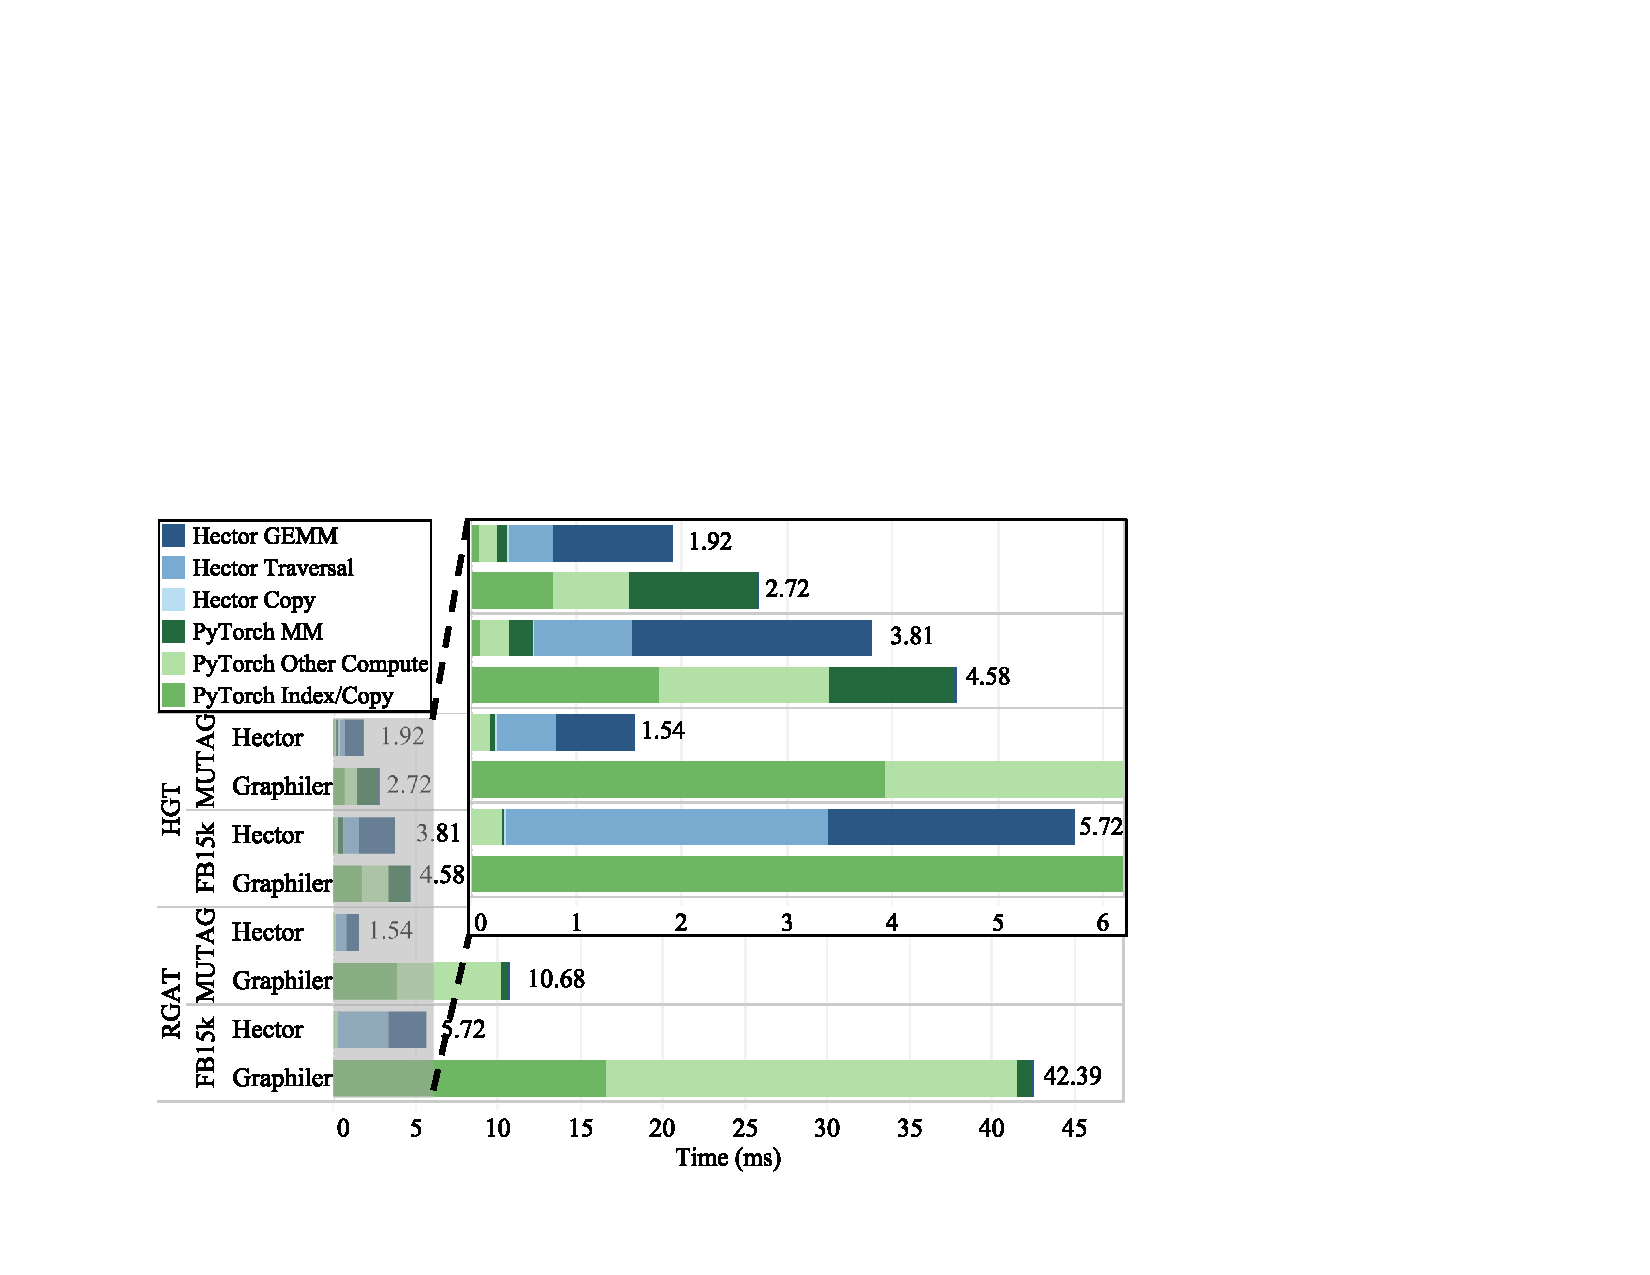
\includegraphics[width=\linewidth]{figures/Hector/BreakdownBGv3.pdf}
\caption{\label{fig:bg_breakdown} Breakdown of inference time by Graphiler and Hector. Matrix multiply~(MM) includes SpMM. We categorize PyTorch time not accounted for by kernels as ``PyTorch Other Compute''.} 
\end{figure}




\subsection{Inefficiency in Existing Computation Stack: A Case Study on Edgewise Typed Linear Layers}
\label{sec:segmentmm}

We use an edgewise typed linear layer as an example to walk through the various performance overheads in the existing computation stack, as summarized in Figure~\ref{fig:inefficient_stack}. 
Edgewise typed linear layer applies a typed linear operator on each edge to one of its vectors. The weight of the linear operator used in the computation depends on each edge's type. For example, the edge message in an RGCN layer~(Figure~\ref{fig:rgnn_layer}) or an RGAT layer~(Figure~\ref{fig:rgat_layer}), is produced by a typed linear layer.

\begin{figure}[!t]
\centering
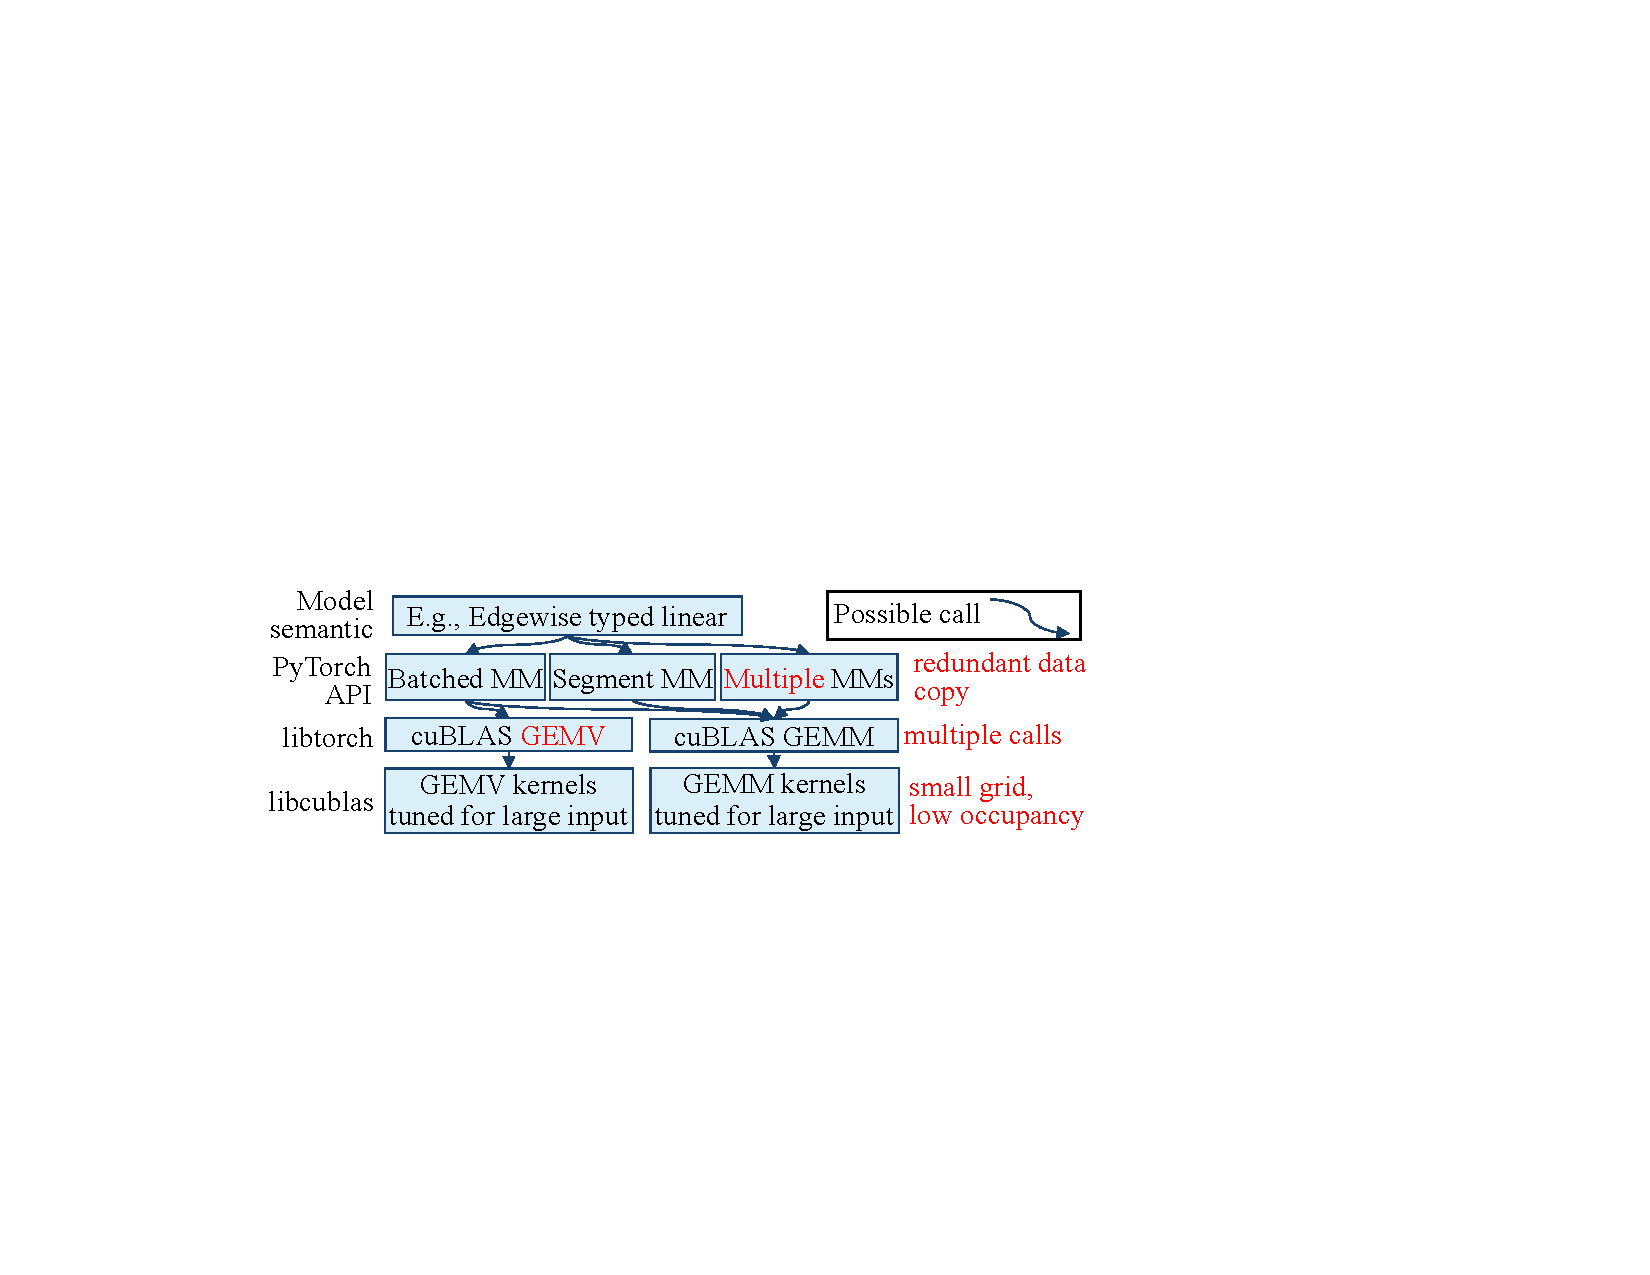
\includegraphics[width=0.8\linewidth]{figures/Hector/StackInefficiencyCompactv3.compact.pdf}
\caption{\label{fig:inefficient_stack} Inefficiency~(in red) exists in all layers of existing systems.}
\end{figure}

A typed linear layer is typically implemented using batched matrix multiply~(BMM) or segment matrix multiply~(segment MM)~\cite{isratsegmm}. 
For example, PyG \texttt{FastRGCNConv} implemented typed linear layers using BMM to unleash parallelism. However, a temporary tensor must be created from the weight tensor due to the lack of support for indirect addressing by PyTorch tensor APIs: the typed linear layer could be denoted as  $Y[i,0,j]:=\sum_k(X[i,0,k]\times W[T[i],k,j])$ where $X[i,0,\cdot]$, $Y[i,0,\cdot]$ and $W[T[i],\cdot,\cdot]$ are input feature, output feature of node $i$ and the weight of node $i$'s type. The middle dimension of $X$ and $Y$ are needed to make the operation a matrix multiply. However, there is currently no support for specifying $T[i]$ as one of the arguments to an operator in PyTorch;  
one must create $W^\prime[i,k,j]:=W[T[i],k,j]$ before the typed linear layer.


Segment MM requires presorting features by types. Then,  the node/edge feature tensor is in the form of segments of features of the same type: the segment MM kernel then applies the corresponding weight tensor of the type to each segment. 
If neither BMM nor segment MM can be employed, one may fall back to multiple matrix multiplies, leading to higher device API overhead and GPU under-utilization.




Another type of inefficiency is suboptimal math library calls. PyTorch has routines to handle various scenarios, e.g., a tensor is strided in memory layout or is \texttt{NestedTensor}, a pack of tensors. Consequently, PyTorch sometimes performs BMM by launching multiple general matrix-vector multiplies~(GEMVs) kernels, which also leads to API overhead and GPU under-utilization. 



Lastly,  CUDA math libraries were initially developed for large inputs and may not be {efficient} for small inputs~\cite{nvidiaCublasgemmBatchedCuBLASDocuemntation}.

To better illustrate the points, Figure~\ref{fig:bg_breakdown} breaks down HGT and RGAT inference time on FB15k and MUTAG.
Section~\ref{sec:eval_methodology} details the system configurations and datasets.
This experiment measured Graphiler~\cite{xieGraphilerCompilerGraph}, which executed compiled TorchScript code and delivered the best inference performance among the existing systems tested in Hector.
Figure~\ref{fig:bg_breakdown} shows that indexing and copying take up a significant portion, and the portion of GEMM operations, i.e., MM vs. Other compute,  varied with graphs.
By profiling, we found that the CUDA API overhead is 22\% of the time of the critical path, which is the sum of the API overhead and kernel duration. This is partly due to a huge number of kernel launches caused by 1)~libraries calling a series of kernels to fulfill an API invocation and 2)~some operators calling separate sets of kernels for each types in the graph.



In contrast, Hector 1)~\textbf{lowers more of the logic to GEMM}, 
and 2)~assembles kernels with flexible access schemes to \textbf{gather and scatter data on the fly} to eliminate redundant data movement. Consequently, Hector does not replicate weights during computation. As shown, \textbf{this strategy achieves better performance than using hand-optimized kernels with dedicated functions to data movement, e.g., in Graphiler}.



To address the performance challenges in RGNN systems due to both RGNN's inherent computation pattern and the system design, we propose the Hector IR and code generation framework. By the IR design that \textit{decouples} and \textit{expresses} the model semantics, data layout, and operator-specific schedules, Hector opens up these opportunities and the integration of all three aspects into the design space.
Table~\ref{tab:salesman_matrix} shows the feature comparison of Hector with existing systems. 

\begin{table}[!htbp]
\centering
\begin{tabular}{@{}llllll@{}}
\toprule
&                                & \rotatebox{75}{Graphiler} & \rotatebox{75}{Seastar}   & \rotatebox{75}{HGL}       & \rotatebox{75}{\textbf{Hector}}   \\ \midrule
\multirow{2}{*}{\textbf{Target}}                                                 & \textbf{Inference}             & \Checkmark & \Checkmark &           & \Checkmark       \\
& \textbf{Training}              &           & \Checkmark & \Checkmark & \Checkmark       \\\cline{1-2}
\multicolumn{2}{@{}l}{\textbf{Memory efficiency}}                          & \Checkmark &           & \Checkmark & \textbf{better} \\\cline{1-2}
\multirow{3}{*}{\textbf{\begin{tabular}[c]{@{}l@{}}Design\\ space\end{tabular}}} & \textbf{Data layout}           &           &           &           & \Checkmark       \\
& \textbf{Intra-operator schedule}     &           &           &           & \Checkmark       \\
& \textbf{Inter-operator optimization} & \Checkmark & \Checkmark & \Checkmark & \Checkmark       \\ \bottomrule
\end{tabular}
\caption{Features of Hector and prior~\cite{xieGraphilerCompilerGraph, wuSeastarVertexcentricProgramming2021, guiHGLAcceleratingHeterogeneous} GNN compilers.\label{tab:salesman_matrix}
}
\end{table}

